% 2011 年福建卷文科第 15 题：正方体与 AD 中点 E、CD 上点 F。
% 来源 PDF：普通高考/2011/2011福建文.pdf，SHA-256 e649bdc736a215d4e41e02c6a7945953aca84a87a23e6a903596d61025cdf322。
% 原页：第 1 页第 2 栏下部，书页码 661。示意。
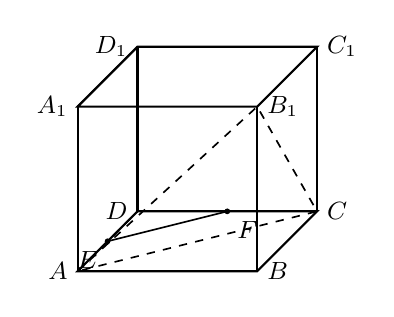
\begin{tikzpicture}[>=stealth, semithick, font=\small, scale=0.95]
  \coordinate (A) at (0,0); \coordinate (B) at (2.4,0);
  \coordinate (C) at (3.2,0.8); \coordinate (D) at (0.8,0.8);
  \coordinate (A1) at (0,2.2); \coordinate (B1) at (2.4,2.2);
  \coordinate (C1) at (3.2,3.0); \coordinate (D1) at (0.8,3.0);
  \coordinate (E) at (0.4,0.4); \coordinate (F) at (2.0,0.8);
  \draw[thick] (A)--(B)--(C)--(D)--cycle;
  \draw[thick] (A1)--(B1)--(C1)--(D1)--cycle;
  \draw[thick] (A)--(A1) (B)--(B1) (C)--(C1) (D)--(D1);
  \draw[dashed] (A)--(D) (D)--(D1) (A1)--(D1);
  \draw (E)--(F);
  \draw[dashed] (A)--(B1)--(C)--(A);
  \fill (E) circle (1.1pt) node[below left] {$E$};
  \fill (F) circle (1.1pt) node[below right] {$F$};
  \node[left] at (A) {$A$}; \node[right] at (B) {$B$};
  \node[right] at (C) {$C$}; \node[left] at (D) {$D$};
  \node[left] at (A1) {$A_1$}; \node[right] at (B1) {$B_1$};
  \node[right] at (C1) {$C_1$}; \node[left] at (D1) {$D_1$};
\end{tikzpicture}
